% Classes of src/models/Therminator3 and their dependencies. Paper: section "Therminator3" (fig:therminator);
% Doxygen: Therminator3.hpp.
%   pdflatex Therminator3Classes.tex; pdftoppm -r 200 -png -singlefile Therminator3Classes.pdf Therminator3Classes;
%   pdftocairo -svg Therminator3Classes.pdf Therminator3Classes.svg
\documentclass[tikz,border=2pt]{standalone}
% Shared style of the class diagrams of CAP (figures/*Classes.tex): \input after \documentclass[tikz]{standalone}.
%  - boxes: blue = abstract base class, light blue = class, green = entry class of the folder (steering class, task),
%    yellow = free functions (tools), grey = class of another folder;
%  - arrows: open triangle = inherits from; dashed with diamond = owns (holds); dashed with arrow = uses.
\usepackage[scaled=0.92]{helvet}
\usetikzlibrary{arrows.meta,shapes.multipart,positioning,fit,backgrounds,calc}
\renewcommand{\familydefault}{\sfdefault}
\definecolor{abstract}{HTML}{D6E4F5}
\definecolor{concrete}{HTML}{EEF4FB}
\definecolor{steer}{HTML}{DCEFD9}
\definecolor{tools}{HTML}{FFF8E6}
\definecolor{external}{HTML}{E9E9E9}
\definecolor{dependline}{HTML}{8A6D3B}
\definecolor{folder}{HTML}{F7F7F7}
\tikzset{
  every picture/.style={font=\scriptsize},
  cls/.style={draw, fill=concrete, align=center, inner sep=2.5pt, text width=#1, font=\tiny},
  cls/.default=3.0cm,
  abs/.style={cls=#1, fill=abstract},
  abs/.default=3.0cm,
  steer/.style={cls=#1, fill=steer, line width=0.8pt},
  steer/.default=4.2cm,
  tool/.style={cls=#1, fill=tools},
  tool/.default=4.2cm,
  ext/.style={cls=#1, fill=external, dashed},
  ext/.default=2.6cm,
  fam/.style={draw, rectangle split, rectangle split parts=2, rectangle split part fill={#1,white},
              rectangle split part align={center,left}, inner sep=2.5pt, align=left},
  inherit/.style={-{Triangle[open,length=2.2mm,width=2.2mm]}, thin},
  uses/.style={dashed, dependline, -{Stealth[length=1.6mm]}, thin},
  owns/.style={dashed, dependline, {Diamond[length=2.4mm,width=1.6mm]}-, thin},
  lbl/.style={font=\tiny, text=dependline, align=center},
  note/.style={font=\tiny, align=left, text=black!70},
  title/.style={font=\footnotesize\bfseries, anchor=north west},
}
% a member line in a class box
\newcommand{\m}[1]{\\#1}
\newcommand{\cn}[1]{{\scriptsize\textbf{#1}}}
\newcommand{\an}[1]{{\scriptsize\textbf{\textit{#1}}}}

% legend common to the class diagrams (place with \legendat{x}{y})
\newcommand{\legendat}[2]{%
  \begin{scope}[shift={(#1,#2)}, font=\tiny]
    \node[abs=0.9cm, minimum height=3mm, inner sep=1pt] (lA) at (0,0) {abstract};
    \node[cls=0.9cm, minimum height=3mm, inner sep=1pt, right=1mm of lA] (lC) {class};
    \node[steer=1.1cm, minimum height=3mm, inner sep=1pt, right=1mm of lC] (lS) {entry class};
    \node[tool=1.1cm, minimum height=3mm, inner sep=1pt, right=1mm of lS] (lT) {functions};
    \node[ext=1.3cm, minimum height=3mm, inner sep=1pt, right=1mm of lT] (lE) {other folder};
    \draw[inherit] ($(lE.east)+(1mm,0)$) -- ++(5mm,0) node[right, inner sep=1pt] (l1) {inherits};
    \draw[owns] ($(l1.east)+(1mm,0)$) -- ++(5mm,0) node[right, inner sep=1pt] (l2) {owns};
    \draw[uses] ($(l2.east)+(1mm,0)$) -- ++(5mm,0) node[right, inner sep=1pt] {uses};
  \end{scope}}

\begin{document}
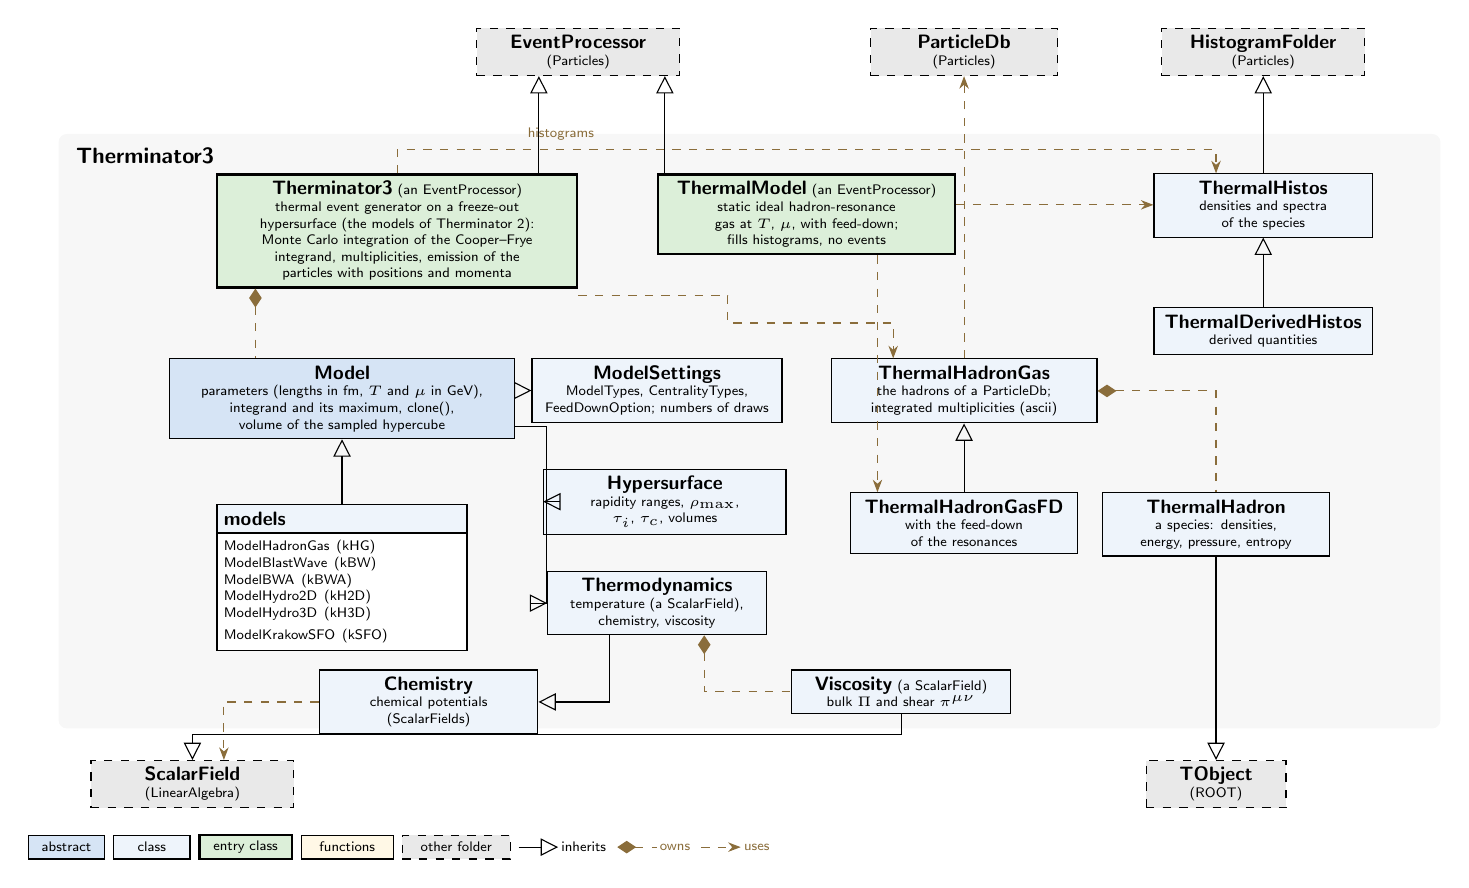
\begin{tikzpicture}[every node/.append style={anchor=north}]
  \begin{scope}[on background layer]
    \fill[folder, rounded corners=3pt] (-0.1,-1.05) rectangle (17.45,-8.6);
  \end{scope}
  \node[title] at (0.0,-1.1) {Therminator3};

  % other folders
  \node[ext=2.4cm] (EP) at (6.5,0.3) {\an{EventProcessor}\m{(Particles)}};
  \node[ext=2.4cm] (HF) at (15.2,0.3) {\an{HistogramFolder}\m{(Particles)}};
  \node[ext=2.2cm] (PDb) at (11.4,0.3) {\cn{ParticleDb}\m{(Particles)}};
  \node[ext=2.4cm] (SF) at (1.6,-9.0) {\cn{ScalarField}\m{(LinearAlgebra)}};
  \node[ext=1.6cm] (TObj) at (14.6,-9.0) {\cn{TObject}\m{(ROOT)}};

  % tasks
  \node[steer=4.4cm] (T3) at (4.2,-1.55)
    {\cn{Therminator3} \tiny(an EventProcessor)\m{thermal event generator on a freeze-out}
     \m{hypersurface (the models of Therminator 2):}\m{Monte Carlo integration of the Cooper--Frye}
     \m{integrand, multiplicities, emission of the}\m{particles with positions and momenta}};
  \node[steer=3.6cm] (TM) at (9.4,-1.55)
    {\cn{ThermalModel} \tiny(an EventProcessor)\m{static ideal hadron-resonance}\m{gas at $T$, $\mu$, with feed-down;}\m{fills histograms, no events}};
  \draw[inherit] (6.0,0 |- T3.north) -- (6.0,0 |- EP.south);
  \draw[inherit] (7.6,0 |- TM.north) -- (7.6,0 |- EP.south);

  % models
  \node[abs=4.2cm] (Model) at (3.5,-3.9)
    {\an{Model}\m{parameters (lengths in fm, $T$ and $\mu$ in GeV),}\m{integrand and its maximum, clone(),}
     \m{volume of the sampled hypercube}};
  \node[fam=concrete, text width=3.0cm] (Models) at (3.5,-5.75)
    {\cn{models}\nodepart{two}\tiny
     ModelHadronGas (kHG)\\ModelBlastWave (kBW)\\ModelBWA (kBWA)\\ModelHydro2D (kH2D)\\ModelHydro3D (kH3D)\\ModelKrakowSFO (kSFO)};
  \draw[inherit] (Models.north) -- (Model.south);
  \draw[owns] (2.4,0 |- T3.south) -- (2.4,0 |- Model.north);

  \node[cls=3.0cm] (Settings) at (7.5,-3.9) {\cn{ModelSettings}\m{ModelTypes, CentralityTypes,}\m{FeedDownOption; numbers of draws}};
  \node[cls=2.9cm] (Hyper) at (7.6,-5.3) {\cn{Hypersurface}\m{rapidity ranges, $\rho_{\max}$,}\m{$\tau_i$, $\tau_c$, volumes}};
  \node[cls=2.6cm] (Thermo) at (7.5,-6.6) {\cn{Thermodynamics}\m{temperature (a ScalarField),}\m{chemistry, viscosity}};
  \node[cls=2.6cm] (Chem) at (4.6,-7.85) {\cn{Chemistry}\m{chemical potentials}\m{(ScalarFields)}};
  \node[cls=2.6cm] (Visc) at (10.6,-7.85) {\cn{Viscosity} \tiny(a ScalarField)\m{bulk $\Pi$ and shear $\pi^{\mu\nu}$}};
  \draw[inherit] (Model.east |- Settings.west) -- (Settings.west);
  \draw[inherit] (Model.east) ++(0,-0.35) -- ++(0.4,0) |- (Hyper.west);
  \draw[inherit] (Model.east) ++(0,-0.35) ++(0.4,0) |- (Thermo.west);
  \draw[inherit] ([xshift=-0.6cm]Thermo.south) |- (Chem.east);
  \draw[owns] ([xshift=0.6cm]Thermo.south) |- (Visc.west);
  \draw[inherit] (Visc.south) -- ++(0,-0.25) -| (SF.north);
  \draw[uses] (Chem.west) -| ([xshift=0.4cm]SF.north);

  % hadrons and histograms
  \node[cls=3.2cm] (Gas) at (11.4,-3.9) {\cn{ThermalHadronGas}\m{the hadrons of a ParticleDb;}\m{integrated multiplicities (ascii)}};
  \node[cls=2.7cm] (GasFD) at (11.4,-5.6) {\cn{ThermalHadronGasFD}\m{with the feed-down}\m{of the resonances}};
  \node[cls=2.7cm] (Hadron) at (14.6,-5.6) {\cn{ThermalHadron}\m{a species: densities,}\m{energy, pressure, entropy}};
  \node[cls=2.6cm] (Histos) at (15.2,-1.55) {\cn{ThermalHistos}\m{densities and spectra}\m{of the species}};
  \node[cls=2.6cm] (DHistos) at (15.2,-3.25) {\cn{ThermalDerivedHistos}\m{derived quantities}};
  \draw[inherit] (GasFD.north) -- (Gas.south);
  \draw[owns] (Gas.east) -| (Hadron.north);
  \draw[uses] (Gas.north) -- (Gas.north |- PDb.south);
  \draw[inherit] (Histos.north) -- (HF.south);
  \draw[inherit] (DHistos.north) -- (Histos.south);
  \draw[inherit] (Hadron.south) -- (Hadron.south |- TObj.north);
  \draw[uses] (T3.east |- 0,-3.1) -- (8.4,-3.1) -- ++(0,-0.35) -| ([xshift=-0.9cm]Gas.north) ;
  \draw[uses] ([xshift=0.9cm]TM.south) -- ([xshift=0.9cm]TM.south |- GasFD.north) ;
  \draw[uses] (TM.east |- 0,-1.95) -- (Histos.west |- 0,-1.95);
  \draw[uses] (T3.north) -- ++(0,0.3) -| node[lbl, pos=0.1, above]{histograms} ([xshift=-0.6cm]Histos.north) ;
  \legendat{0.0}{-9.95}
\end{tikzpicture}
\end{document}
